
\begin{figure}
\centering
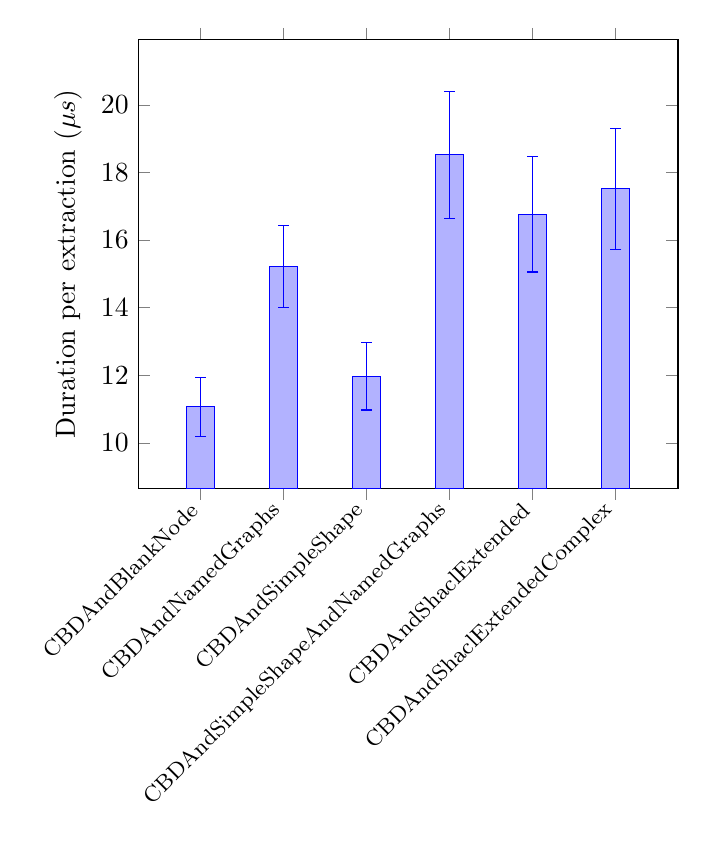
\begin{tikzpicture}
        \begin{axis}[
            ybar,
            enlargelimits=0.15,
            legend style={at={(0.5,-0.15)},
            anchor=north,legend columns=-1},
            ylabel={Duration per extraction ($\mu s$)},
            symbolic x coords={CBDAndBlankNode,CBDAndNamedGraphs,CBDAndSimpleShape,CBDAndSimpleShapeAndNamedGraphs,CBDAndShaclExtended,CBDAndShaclExtendedComplex},
            xtick=data,
            x tick label style={font=\footnotesize,rotate=45, anchor=east},
            nodes near coords align={horizontal},
        ]
            \addplot+[
                error bars/.cd,
                y dir=both,
                y explicit
            ] coordinates {
         (CBDAndBlankNode, 11.063370677196545) +- (0, 0.8712384083996434)
         (CBDAndNamedGraphs, 15.217862123925167) +- (0, 1.2088651348887458)
         (CBDAndSimpleShape, 11.975056336911239) +- (0, 1.0046364406179427)
         (CBDAndSimpleShapeAndNamedGraphs, 18.523247927563368) +- (0, 1.8735627632238423)
         (CBDAndShaclExtended, 16.760628339328065) +- (0, 1.7036244375897358)
         (CBDAndShaclExtendedComplex, 17.51703759120106) +- (0, 1.7942769973185504)

             };
        \end{axis}
    \end{tikzpicture}
    \caption{Graph depicting performance of inband extraction algorithm}
\end{figure}
